% Options for packages loaded elsewhere
\PassOptionsToPackage{unicode}{hyperref}
\PassOptionsToPackage{hyphens}{url}
%
\documentclass[
]{article}
\usepackage{amsmath,amssymb}
\usepackage{lmodern}
\usepackage{ifxetex,ifluatex}
\ifnum 0\ifxetex 1\fi\ifluatex 1\fi=0 % if pdftex
  \usepackage[T1]{fontenc}
  \usepackage[utf8]{inputenc}
  \usepackage{textcomp} % provide euro and other symbols
\else % if luatex or xetex
  \usepackage{unicode-math}
  \defaultfontfeatures{Scale=MatchLowercase}
  \defaultfontfeatures[\rmfamily]{Ligatures=TeX,Scale=1}
\fi
% Use upquote if available, for straight quotes in verbatim environments
\IfFileExists{upquote.sty}{\usepackage{upquote}}{}
\IfFileExists{microtype.sty}{% use microtype if available
  \usepackage[]{microtype}
  \UseMicrotypeSet[protrusion]{basicmath} % disable protrusion for tt fonts
}{}
\makeatletter
\@ifundefined{KOMAClassName}{% if non-KOMA class
  \IfFileExists{parskip.sty}{%
    \usepackage{parskip}
  }{% else
    \setlength{\parindent}{0pt}
    \setlength{\parskip}{6pt plus 2pt minus 1pt}}
}{% if KOMA class
  \KOMAoptions{parskip=half}}
\makeatother
\usepackage{xcolor}
\IfFileExists{xurl.sty}{\usepackage{xurl}}{} % add URL line breaks if available
\IfFileExists{bookmark.sty}{\usepackage{bookmark}}{\usepackage{hyperref}}
\hypersetup{
  pdftitle={Exercícios de R com R Markdown},
  pdfauthor={Rafael Tenfen},
  hidelinks,
  pdfcreator={LaTeX via pandoc}}
\urlstyle{same} % disable monospaced font for URLs
\usepackage[margin=1in]{geometry}
\usepackage{color}
\usepackage{fancyvrb}
\newcommand{\VerbBar}{|}
\newcommand{\VERB}{\Verb[commandchars=\\\{\}]}
\DefineVerbatimEnvironment{Highlighting}{Verbatim}{commandchars=\\\{\}}
% Add ',fontsize=\small' for more characters per line
\usepackage{framed}
\definecolor{shadecolor}{RGB}{248,248,248}
\newenvironment{Shaded}{\begin{snugshade}}{\end{snugshade}}
\newcommand{\AlertTok}[1]{\textcolor[rgb]{0.94,0.16,0.16}{#1}}
\newcommand{\AnnotationTok}[1]{\textcolor[rgb]{0.56,0.35,0.01}{\textbf{\textit{#1}}}}
\newcommand{\AttributeTok}[1]{\textcolor[rgb]{0.77,0.63,0.00}{#1}}
\newcommand{\BaseNTok}[1]{\textcolor[rgb]{0.00,0.00,0.81}{#1}}
\newcommand{\BuiltInTok}[1]{#1}
\newcommand{\CharTok}[1]{\textcolor[rgb]{0.31,0.60,0.02}{#1}}
\newcommand{\CommentTok}[1]{\textcolor[rgb]{0.56,0.35,0.01}{\textit{#1}}}
\newcommand{\CommentVarTok}[1]{\textcolor[rgb]{0.56,0.35,0.01}{\textbf{\textit{#1}}}}
\newcommand{\ConstantTok}[1]{\textcolor[rgb]{0.00,0.00,0.00}{#1}}
\newcommand{\ControlFlowTok}[1]{\textcolor[rgb]{0.13,0.29,0.53}{\textbf{#1}}}
\newcommand{\DataTypeTok}[1]{\textcolor[rgb]{0.13,0.29,0.53}{#1}}
\newcommand{\DecValTok}[1]{\textcolor[rgb]{0.00,0.00,0.81}{#1}}
\newcommand{\DocumentationTok}[1]{\textcolor[rgb]{0.56,0.35,0.01}{\textbf{\textit{#1}}}}
\newcommand{\ErrorTok}[1]{\textcolor[rgb]{0.64,0.00,0.00}{\textbf{#1}}}
\newcommand{\ExtensionTok}[1]{#1}
\newcommand{\FloatTok}[1]{\textcolor[rgb]{0.00,0.00,0.81}{#1}}
\newcommand{\FunctionTok}[1]{\textcolor[rgb]{0.00,0.00,0.00}{#1}}
\newcommand{\ImportTok}[1]{#1}
\newcommand{\InformationTok}[1]{\textcolor[rgb]{0.56,0.35,0.01}{\textbf{\textit{#1}}}}
\newcommand{\KeywordTok}[1]{\textcolor[rgb]{0.13,0.29,0.53}{\textbf{#1}}}
\newcommand{\NormalTok}[1]{#1}
\newcommand{\OperatorTok}[1]{\textcolor[rgb]{0.81,0.36,0.00}{\textbf{#1}}}
\newcommand{\OtherTok}[1]{\textcolor[rgb]{0.56,0.35,0.01}{#1}}
\newcommand{\PreprocessorTok}[1]{\textcolor[rgb]{0.56,0.35,0.01}{\textit{#1}}}
\newcommand{\RegionMarkerTok}[1]{#1}
\newcommand{\SpecialCharTok}[1]{\textcolor[rgb]{0.00,0.00,0.00}{#1}}
\newcommand{\SpecialStringTok}[1]{\textcolor[rgb]{0.31,0.60,0.02}{#1}}
\newcommand{\StringTok}[1]{\textcolor[rgb]{0.31,0.60,0.02}{#1}}
\newcommand{\VariableTok}[1]{\textcolor[rgb]{0.00,0.00,0.00}{#1}}
\newcommand{\VerbatimStringTok}[1]{\textcolor[rgb]{0.31,0.60,0.02}{#1}}
\newcommand{\WarningTok}[1]{\textcolor[rgb]{0.56,0.35,0.01}{\textbf{\textit{#1}}}}
\usepackage{graphicx}
\makeatletter
\def\maxwidth{\ifdim\Gin@nat@width>\linewidth\linewidth\else\Gin@nat@width\fi}
\def\maxheight{\ifdim\Gin@nat@height>\textheight\textheight\else\Gin@nat@height\fi}
\makeatother
% Scale images if necessary, so that they will not overflow the page
% margins by default, and it is still possible to overwrite the defaults
% using explicit options in \includegraphics[width, height, ...]{}
\setkeys{Gin}{width=\maxwidth,height=\maxheight,keepaspectratio}
% Set default figure placement to htbp
\makeatletter
\def\fps@figure{htbp}
\makeatother
\setlength{\emergencystretch}{3em} % prevent overfull lines
\providecommand{\tightlist}{%
  \setlength{\itemsep}{0pt}\setlength{\parskip}{0pt}}
\setcounter{secnumdepth}{-\maxdimen} % remove section numbering
\ifluatex
  \usepackage{selnolig}  % disable illegal ligatures
\fi

\title{Exercícios de R com R Markdown}
\author{Rafael Tenfen}
\date{21/04/2021}

\begin{document}
\maketitle

\hypertarget{descriuxe7uxe3o-da-atividade}{%
\subsection{Descrição da Atividade}\label{descriuxe7uxe3o-da-atividade}}

Nesta atividade você irá realizar algumas análises de dados na forma de
um documento reproduzível com R Markdown. Você deve usar o RStudio para
editar este arquivo .Rmd e processá-lo em um arquivo HTML.

Algumas recomendações:

\begin{itemize}
\tightlist
\item
  Se você não estiver habituado com R Markdown, acostume-se a processar
  com frequência o documento, usando o botão \textbf{Knit}. Isso
  permitirá que eventuais erros no documento ou no código R sejam
  identificados rapidamente, pouco depois de terem sido cometidos, o que
  facilitará sua correção. Na verdade, é uma boa ideia você fazer isso
  \textbf{agora}, para garantir que seu ambiente esteja configurado
  corretamente. Se você receber uma mensagem de erro do tipo
  \texttt{Error\ in\ library(foo)}, isso significa que o pacote
  \texttt{foo} não está instalado. Para instalar um pacote, execute o
  comando \texttt{install.packages("foo")} no Console, ou clique em
  \emph{Tools} -\textgreater{} \emph{Install Packages}.
\item
  \textbf{Não esqueça} de colocar seu nome e a data no cabeçalho do
  arquivo .Rmd (onde diz ``Insira seu nome aqui'' e ``Insira a data'').
\item
  As variáveis usadas no código R devem ser usadas para tornar o
  relatório mais reproduzível, eliminando uma fonte de erros. Em vez de
  copiar valores manualmente, atribua os resultados a variáveis e
  exiba-os usando
  \href{https://bookdown.org/yihui/rmarkdown-cookbook/r-code.html}{código
  R \emph{inline}}. Por exemplo, nas respostas você pode escrever algo
  como
\end{itemize}

\begin{Shaded}
\begin{Highlighting}[]
\NormalTok{Os tempos de execução ficam entre }\StringTok{\textasciigrave{}}\AttributeTok{r texec.min}\StringTok{\textasciigrave{}}\NormalTok{ e }\StringTok{\textasciigrave{}}\AttributeTok{r texec.max}\StringTok{\textasciigrave{}}\NormalTok{ ms.}
\end{Highlighting}
\end{Shaded}

\begin{itemize}
\tightlist
\item
  Após concluir a atividade, você deverá submeter no Moodle um arquivo
  ZIP contendo:

  \begin{itemize}
  \tightlist
  \item
    o arquivo fonte .Rmd;
  \item
    a saída processada (PDF ou HTML) do arquivo .Rmd;
  \item
    outros arquivos necessários ao processamento do arquivo .Rmd (se
    houver).
  \end{itemize}
\end{itemize}

\hypertarget{anuxe1lise-de-tempos-de-execuuxe7uxe3o}{%
\subsection{Análise de Tempos de
Execução}\label{anuxe1lise-de-tempos-de-execuuxe7uxe3o}}

O primeiro exercício consiste em analisar os dados de 92 tempos de
execução de uma sub-rotina contidos no arquivo \texttt{texec-iops.dat}.
Cada linha do arquivo representa uma execução, para a qual foram
coletadas duas métricas:

\begin{itemize}
\tightlist
\item
  \texttt{texec}: tempo de execução da sub-rotina, em ms;
\item
  \texttt{iops}: quantidade de operações de entrada/saída realizadas
  pela sub-rotina.
\end{itemize}

Analise os dados e responda às seguintes questões:

\begin{enumerate}
\def\labelenumi{\arabic{enumi}.}
\tightlist
\item
  Qual o maior e o menor tempo de execução registrados?
\item
  Qual o tempo médio de execução?
\item
  Qual é a mediana do número de operações de E/S?
\item
  Em quantas execuções não foi realizada nenhuma operação de E/S?
\item
  Quantas execuções levaram 300 ms ou mais para executar? Qual o número
  médio de operações de E/S dessas execuções?
\item
  Gere um gráfico de dispersão do tempo de execução em função do número
  de operações de E/S (ou seja, o eixo \emph{x} é o número de operações
  e o eixo \emph{y} é o tempo de execução). De que maneira o número de
  operações de E/S influencia o tempo de execução?
\end{enumerate}

\begin{quote}
Neste exercício, o código R está parcialmente escrito abaixo. Como ele
tem algumas lacunas que precisam ser preenchidas, ele não pode ser
executado como está. Você só precisa fazer duas coisas: (1) completar as
lacunas no código e (2) mudar \texttt{eval} no cabeçalho do bloco
(\emph{chunk}) para \texttt{TRUE} para que ele seja executado quando
você processar o documento com \textbf{Knit}.
\end{quote}

Código e saídas do R:

\begin{Shaded}
\begin{Highlighting}[]
\CommentTok{\# le os dados do arquivo para o data frame dados}
\NormalTok{dados }\OtherTok{\textless{}{-}} \FunctionTok{read.table}\NormalTok{(}\StringTok{"texec{-}iops.dat"}\NormalTok{, }\AttributeTok{header =} \ConstantTok{TRUE}\NormalTok{)}

\CommentTok{\# 1}
\CommentTok{\# texec.min é o menor elemento da coluna texec}
\NormalTok{texec.min }\OtherTok{\textless{}{-}} \FunctionTok{min}\NormalTok{(dados}\SpecialCharTok{$}\NormalTok{texec)}
\CommentTok{\# texec.max é o maior elemento da coluna texec}
\NormalTok{texec.max }\OtherTok{\textless{}{-}} \FunctionTok{max}\NormalTok{(dados}\SpecialCharTok{$}\NormalTok{texec) }

\CommentTok{\# 2}
\CommentTok{\# texec.avg é a média de texec}
\NormalTok{texec.avg }\OtherTok{\textless{}{-}} \FunctionTok{mean}\NormalTok{(dados}\SpecialCharTok{$}\NormalTok{texec) }
\CommentTok{\# arredonda para uma casa decimal}
\NormalTok{texec.avg }\OtherTok{\textless{}{-}} \FunctionTok{round}\NormalTok{(texec.avg, }\DecValTok{1}\NormalTok{)}

\CommentTok{\# 3}
\CommentTok{\# iops.med é a mediana da coluna iops}
\NormalTok{iops.med }\OtherTok{\textless{}{-}} \FunctionTok{median}\NormalTok{(dados}\SpecialCharTok{$}\NormalTok{iops)}

\CommentTok{\# 4}
\CommentTok{\# iops.0 é o número de valores 0 em iops}
\NormalTok{iops}\FloatTok{.0} \OtherTok{\textless{}{-}} \FunctionTok{length}\NormalTok{(dados}\SpecialCharTok{$}\NormalTok{iops[dados}\SpecialCharTok{$}\NormalTok{iops }\SpecialCharTok{==} \DecValTok{0}\NormalTok{])}

\CommentTok{\# 5}
\CommentTok{\# dados.300 contém apenas as linhas com texec mínimo de 300}
\CommentTok{\# iops.300.avg é a média de iops em dados.300}
\NormalTok{dados}\FloatTok{.300} \OtherTok{\textless{}{-}}\NormalTok{ dados[dados}\SpecialCharTok{$}\NormalTok{texec }\SpecialCharTok{\textgreater{}=} \DecValTok{300}\NormalTok{,]}
\NormalTok{iops.}\FloatTok{300.}\NormalTok{avg }\OtherTok{\textless{}{-}} \FunctionTok{mean}\NormalTok{(dados}\FloatTok{.300}\SpecialCharTok{$}\NormalTok{iops)}
\NormalTok{iops.}\FloatTok{300.}\NormalTok{avg }\OtherTok{\textless{}{-}} \FunctionTok{round}\NormalTok{(iops.}\FloatTok{300.}\NormalTok{avg, }\DecValTok{1}\NormalTok{)   }\CommentTok{\# arredonda para uma casa decimal}

\CommentTok{\# 6}
\FunctionTok{with}\NormalTok{(dados, }\FunctionTok{plot}\NormalTok{(dados}\SpecialCharTok{$}\NormalTok{iops, dados}\SpecialCharTok{$}\NormalTok{texec))}
\end{Highlighting}
\end{Shaded}

\begin{center}\includegraphics[width=0.75\linewidth]{ex-r-markdown_files/figure-latex/analise-texec-1} \end{center}

Respostas:

\begin{enumerate}
\def\labelenumi{\arabic{enumi}.}
\tightlist
\item
  Resposta da questão 1:
\end{enumerate}

\begin{itemize}
\tightlist
\item
  Maior tempo: 480
\item
  Menor tempo: 71
\end{itemize}

\begin{enumerate}
\def\labelenumi{\arabic{enumi}.}
\setcounter{enumi}{1}
\tightlist
\item
  Resposta da questão 2:
\end{enumerate}

\begin{itemize}
\tightlist
\item
  Tempo médio de execução: 6
\end{itemize}

\begin{enumerate}
\def\labelenumi{\arabic{enumi}.}
\setcounter{enumi}{2}
\tightlist
\item
  Resposta da questão 3:
\end{enumerate}

\begin{itemize}
\tightlist
\item
  Mediana: 6
\end{itemize}

\begin{enumerate}
\def\labelenumi{\arabic{enumi}.}
\setcounter{enumi}{3}
\tightlist
\item
  Resposta da questão 4:
\end{enumerate}

\begin{itemize}
\tightlist
\item
  Em 5 execuções não foi realizada nenhuma operação
\end{itemize}

\begin{enumerate}
\def\labelenumi{\arabic{enumi}.}
\setcounter{enumi}{4}
\tightlist
\item
  Resposta da questão 5:
\end{enumerate}

\begin{itemize}
\tightlist
\item
  8 execuções levaram 300ms ou mais para executar
\item
  24.5 e a media do numero de operaçoes
\end{itemize}

\begin{enumerate}
\def\labelenumi{\arabic{enumi}.}
\setcounter{enumi}{5}
\tightlist
\item
  Resposta da questão 6:
\end{enumerate}

\begin{Shaded}
\begin{Highlighting}[]
\FunctionTok{with}\NormalTok{(dados, }\FunctionTok{plot}\NormalTok{(dados}\SpecialCharTok{$}\NormalTok{iops, dados}\SpecialCharTok{$}\NormalTok{texec))}
\end{Highlighting}
\end{Shaded}

\begin{center}\includegraphics[width=0.75\linewidth]{ex-r-markdown_files/figure-latex/unnamed-chunk-2-1} \end{center}

\begin{itemize}
\tightlist
\item
  O tempo de execução tende a aumentar de acordo com número de
  operações.
\end{itemize}

\hypertarget{anuxe1lise-do-conjunto-mtcars}{%
\subsection{\texorpdfstring{Análise do conjunto
\texttt{mtcars}}{Análise do conjunto mtcars}}\label{anuxe1lise-do-conjunto-mtcars}}

Diversos conjuntos de dados podem ser encontrados em qualquer instalação
de R, e podem ser acessados diretamente pelo seu nome.\footnote{O
  comando \texttt{data()} mostra uma lista dos conjuntos disponíveis.}
Um deles é \texttt{mtcars}, que traz 11 características de 32 carros
publicadas na revista americana \emph{Motor Trend}. Você pode visualizar
o conjunto com \texttt{View(mtcars)}, e consultar a descrição de cada
variável usando o comando \texttt{?mtcars}. Neste exercício você irá
analisar algumas dessas variáveis.

Usando o conjunto \texttt{mtcars}, responda às seguintes questões:

\begin{enumerate}
\def\labelenumi{\arabic{enumi}.}
\tightlist
\item
  A variável \texttt{hp} representa a potência do motor. Qual carro tem
  o motor mais potente, e qual é a sua potência? E o motor menos
  potente?
\item
  A variável \texttt{am} indica o tipo de transmissão (0=automática,
  1=manual). Qual carro com transmissão automática é o mais potente?
\item
  A variável \texttt{mpg} representa o consumo de combustível (em milhas
  por galão, 1 mpg = 0,425 km/l). É possível afirmar que o consumo médio
  de carros automáticos é maior que, menor que, ou igual ao consumo de
  carros com transmissão manual?
\item
  Quais carros possuem consumo igual ou melhor que 12 km/l?
\item
  A variável \texttt{qsec} representa o tempo (em segundos) para
  percorrer 1/4 de milha, e a variável \texttt{vs} indica a disposição
  dos cilindros do motor (0=cilindros em V, 1=cilindros em linha). Com
  base nos dados, é possível afirmar que motores com cilindros em V têm
  melhor desempenho (em termos de \texttt{qsec}) do que motores com
  cilndros em linha?
\item
  A variável \texttt{wt} representa o peso (em milhares de libras). Com
  base nos dados, como você diria que o peso afeta o consumo? (Dica:
  faça um gráfico de dispersão de consumo x peso.)
\item
  A variável \texttt{gear} representa o número de marchas. Com bsae nos
  dados, é possível afirmar que carros com mais marchas são mais (ou
  menos) potentes?
\end{enumerate}

Código e saídas do R:

\begin{Shaded}
\begin{Highlighting}[]
\CommentTok{\# seu codigo R vai aqui}
\NormalTok{mtcars.hp.max }\OtherTok{\textless{}{-}} \FunctionTok{max}\NormalTok{(mtcars}\SpecialCharTok{$}\NormalTok{hp)}
\NormalTok{mtcars.hp.min }\OtherTok{\textless{}{-}} \FunctionTok{min}\NormalTok{(mtcars}\SpecialCharTok{$}\NormalTok{hp)}

\NormalTok{mtcars.hp.maxcar }\OtherTok{\textless{}{-}}\NormalTok{ mtcars[mtcars}\SpecialCharTok{$}\NormalTok{hp }\SpecialCharTok{==}\NormalTok{ mtcars.hp.max,]}
\NormalTok{mtcars.hp.mincar }\OtherTok{\textless{}{-}}\NormalTok{ mtcars[mtcars}\SpecialCharTok{$}\NormalTok{hp }\SpecialCharTok{==}\NormalTok{ mtcars.hp.min,]}

\NormalTok{mtcars.automatic }\OtherTok{\textless{}{-}}\NormalTok{ mtcars[mtcars}\SpecialCharTok{$}\NormalTok{am }\SpecialCharTok{==} \DecValTok{0}\NormalTok{,]}
\NormalTok{mtcars.automatic.hp.maxcar }\OtherTok{\textless{}{-}}\NormalTok{ mtcars.automatic[mtcars.automatic}\SpecialCharTok{$}\NormalTok{hp }\SpecialCharTok{==} \FunctionTok{max}\NormalTok{(mtcars.automatic}\SpecialCharTok{$}\NormalTok{hp),]}

\NormalTok{mtcars.manual }\OtherTok{\textless{}{-}}\NormalTok{ mtcars[mtcars}\SpecialCharTok{$}\NormalTok{am }\SpecialCharTok{==} \DecValTok{1}\NormalTok{,]}
\NormalTok{mtcars.automatic.meanmpg }\OtherTok{\textless{}{-}} \FunctionTok{mean}\NormalTok{(mtcars.automatic}\SpecialCharTok{$}\NormalTok{mpg)}
\NormalTok{mtcars.manual.meanmpg }\OtherTok{\textless{}{-}} \FunctionTok{mean}\NormalTok{(mtcars.manual}\SpecialCharTok{$}\NormalTok{mpg)}

\NormalTok{mtcars.meanmpg.txt }\OtherTok{\textless{}{-}} \StringTok{\textquotesingle{}Maior\textquotesingle{}} \CommentTok{\# is default}
\ControlFlowTok{if}\NormalTok{ (mtcars.automatic.meanmpg }\SpecialCharTok{==}\NormalTok{ mtcars.manual.meanmpg) \{}
\NormalTok{  mtcars.meanmpg.txt }\OtherTok{\textless{}{-}} \StringTok{\textquotesingle{}Igual\textquotesingle{}}
\NormalTok{\}}

\ControlFlowTok{if}\NormalTok{ (mtcars.automatic.meanmpg }\SpecialCharTok{\textgreater{}}\NormalTok{ mtcars.manual.meanmpg) \{}
\NormalTok{  mtcars.bigger.meanmpg }\OtherTok{\textless{}{-}} \StringTok{\textquotesingle{}Automáticos\textquotesingle{}}
\NormalTok{  mtcars.minor.meanmpg }\OtherTok{\textless{}{-}} \StringTok{\textquotesingle{}Manuais\textquotesingle{}}
\NormalTok{\} }\ControlFlowTok{else}\NormalTok{ \{}
\NormalTok{  mtcars.bigger.meanmpg }\OtherTok{\textless{}{-}} \StringTok{\textquotesingle{}Manuais\textquotesingle{}}
\NormalTok{  mtcars.minor.meanmpg }\OtherTok{\textless{}{-}} \StringTok{\textquotesingle{}Automáticos\textquotesingle{}}
\NormalTok{\}}

\NormalTok{mpg\_kg }\OtherTok{\textless{}{-}} \FloatTok{0.425}
\NormalTok{km\_l\_12 }\OtherTok{\textless{}{-}} \DecValTok{12} \SpecialCharTok{/}\NormalTok{ mpg\_kg}
\NormalTok{mtcars.mpg.km\_l\_12 }\OtherTok{\textless{}{-}}\NormalTok{ mtcars[mtcars}\SpecialCharTok{$}\NormalTok{mpg }\SpecialCharTok{\textgreater{}=}\NormalTok{ km\_l\_12,]}

\NormalTok{mtcars.vs.v }\OtherTok{\textless{}{-}}\NormalTok{ mtcars[mtcars}\SpecialCharTok{$}\NormalTok{vs }\SpecialCharTok{==} \DecValTok{0}\NormalTok{,]}
\NormalTok{mtcars.vs.line }\OtherTok{\textless{}{-}}\NormalTok{ mtcars[mtcars}\SpecialCharTok{$}\NormalTok{vs }\SpecialCharTok{==} \DecValTok{1}\NormalTok{,]}

\NormalTok{mtcars.vs.v.mean }\OtherTok{\textless{}{-}} \FunctionTok{mean}\NormalTok{(mtcars.vs.v}\SpecialCharTok{$}\NormalTok{qsec)}
\NormalTok{mtcars.vs.line.mean }\OtherTok{\textless{}{-}} \FunctionTok{mean}\NormalTok{(mtcars.vs.line}\SpecialCharTok{$}\NormalTok{qsec)}

\NormalTok{mtcars.vs.type }\OtherTok{\textless{}{-}} \StringTok{\textquotesingle{}Maior\textquotesingle{}}
\ControlFlowTok{if}\NormalTok{ (mtcars.vs.line.mean }\SpecialCharTok{==}\NormalTok{ mtcars.vs.v.mean) \{}
\NormalTok{  mtcars.vs.type }\OtherTok{\textless{}{-}} \StringTok{\textquotesingle{}Igual\textquotesingle{}}
\NormalTok{\}}

\ControlFlowTok{if}\NormalTok{ (mtcars.vs.line.mean }\SpecialCharTok{\textless{}}\NormalTok{ mtcars.vs.v.mean) \{}
\NormalTok{  mtcars.bigger.qsecmean }\OtherTok{\textless{}{-}} \StringTok{\textquotesingle{}V\textquotesingle{}}
\NormalTok{  mtcars.minor.qsecmean }\OtherTok{\textless{}{-}} \StringTok{\textquotesingle{}Linha\textquotesingle{}}
\NormalTok{\} }\ControlFlowTok{else}\NormalTok{ \{}
\NormalTok{  mtcars.bigger.qsecmean }\OtherTok{\textless{}{-}} \StringTok{\textquotesingle{}Linha\textquotesingle{}}
\NormalTok{  mtcars.minor.qsecmean }\OtherTok{\textless{}{-}} \StringTok{\textquotesingle{}V\textquotesingle{}}
\NormalTok{\}}

\FunctionTok{with}\NormalTok{(mtcars, }\FunctionTok{plot}\NormalTok{(mtcars}\SpecialCharTok{$}\NormalTok{mpg, mtcars}\SpecialCharTok{$}\NormalTok{wt))}
\end{Highlighting}
\end{Shaded}

\begin{center}\includegraphics[width=0.75\linewidth]{ex-r-markdown_files/figure-latex/analise-mtcars-1} \end{center}

\begin{Shaded}
\begin{Highlighting}[]
\FunctionTok{with}\NormalTok{(mtcars, }\FunctionTok{plot}\NormalTok{(mtcars}\SpecialCharTok{$}\NormalTok{gear, mtcars}\SpecialCharTok{$}\NormalTok{hp, }\AttributeTok{type =} \StringTok{\textquotesingle{}h\textquotesingle{}}\NormalTok{, }\AttributeTok{lwd =} \DecValTok{50}\NormalTok{))}
\end{Highlighting}
\end{Shaded}

\begin{center}\includegraphics[width=0.75\linewidth]{ex-r-markdown_files/figure-latex/analise-mtcars-2} \end{center}

\begin{Shaded}
\begin{Highlighting}[]
\NormalTok{gears }\OtherTok{\textless{}{-}} \FunctionTok{sort}\NormalTok{(}\FunctionTok{unique}\NormalTok{(mtcars}\SpecialCharTok{$}\NormalTok{gear))}
\end{Highlighting}
\end{Shaded}

Respostas:

\begin{enumerate}
\def\labelenumi{\arabic{enumi}.}
\tightlist
\item
  Resposta da questão 1
\end{enumerate}

\begin{itemize}
\tightlist
\item
  O carro mais pontente é o Maserati Bora
\item
  O carro menos potente é o Honda Civic
\end{itemize}

\begin{enumerate}
\def\labelenumi{\arabic{enumi}.}
\setcounter{enumi}{1}
\tightlist
\item
  Resposta da questão 2
\end{enumerate}

\begin{itemize}
\tightlist
\item
  Os carros com a transmissão automática mais potente são os Duster 360,
  Camaro Z28
\end{itemize}

\begin{enumerate}
\def\labelenumi{\arabic{enumi}.}
\setcounter{enumi}{2}
\tightlist
\item
  Resposta da questão 3
\end{enumerate}

\begin{itemize}
\tightlist
\item
  A média de consumo dos carros manuais é de 24.3923077
\item
  A média de consumo dos carros automáticos é de 17.1473684
\item
  Os carros Manuais tem uma média de consumo Maior do que os Automáticos
\end{itemize}

\begin{enumerate}
\def\labelenumi{\arabic{enumi}.}
\setcounter{enumi}{3}
\tightlist
\item
  Resposta da questão 4
\end{enumerate}

\begin{itemize}
\tightlist
\item
  Os carros que possuem consumo igual ou maior que 12 km/l são: Fiat
  128, Honda Civic, Toyota Corolla, Lotus Europa
\end{itemize}

\begin{enumerate}
\def\labelenumi{\arabic{enumi}.}
\setcounter{enumi}{4}
\tightlist
\item
  Resposta da questão 5
\end{enumerate}

\begin{itemize}
\tightlist
\item
  A média do tempo em segundos para percorrer 1/4 de milha dos carros de
  cilindro v é 16.6938889
\item
  A média do tempo em segundos para percorrer 1/4 de milha dos carros de
  cilindro em linha é 19.3335714
\item
  Os carros com cilindro em Linha tem a média do tempo em segundos Maior
  do que os de cilindro V para percorrer 1/4 de milha. Então, na média
  os carros com cilindro V tem um desempenho melhor que os de cilindro
  Linha
\end{itemize}

\begin{enumerate}
\def\labelenumi{\arabic{enumi}.}
\setcounter{enumi}{5}
\tightlist
\item
  Resposta da questão 6
\end{enumerate}

\begin{Shaded}
\begin{Highlighting}[]
\FunctionTok{with}\NormalTok{(mtcars, }\FunctionTok{plot}\NormalTok{(mtcars}\SpecialCharTok{$}\NormalTok{mpg, mtcars}\SpecialCharTok{$}\NormalTok{wt))}
\end{Highlighting}
\end{Shaded}

\begin{center}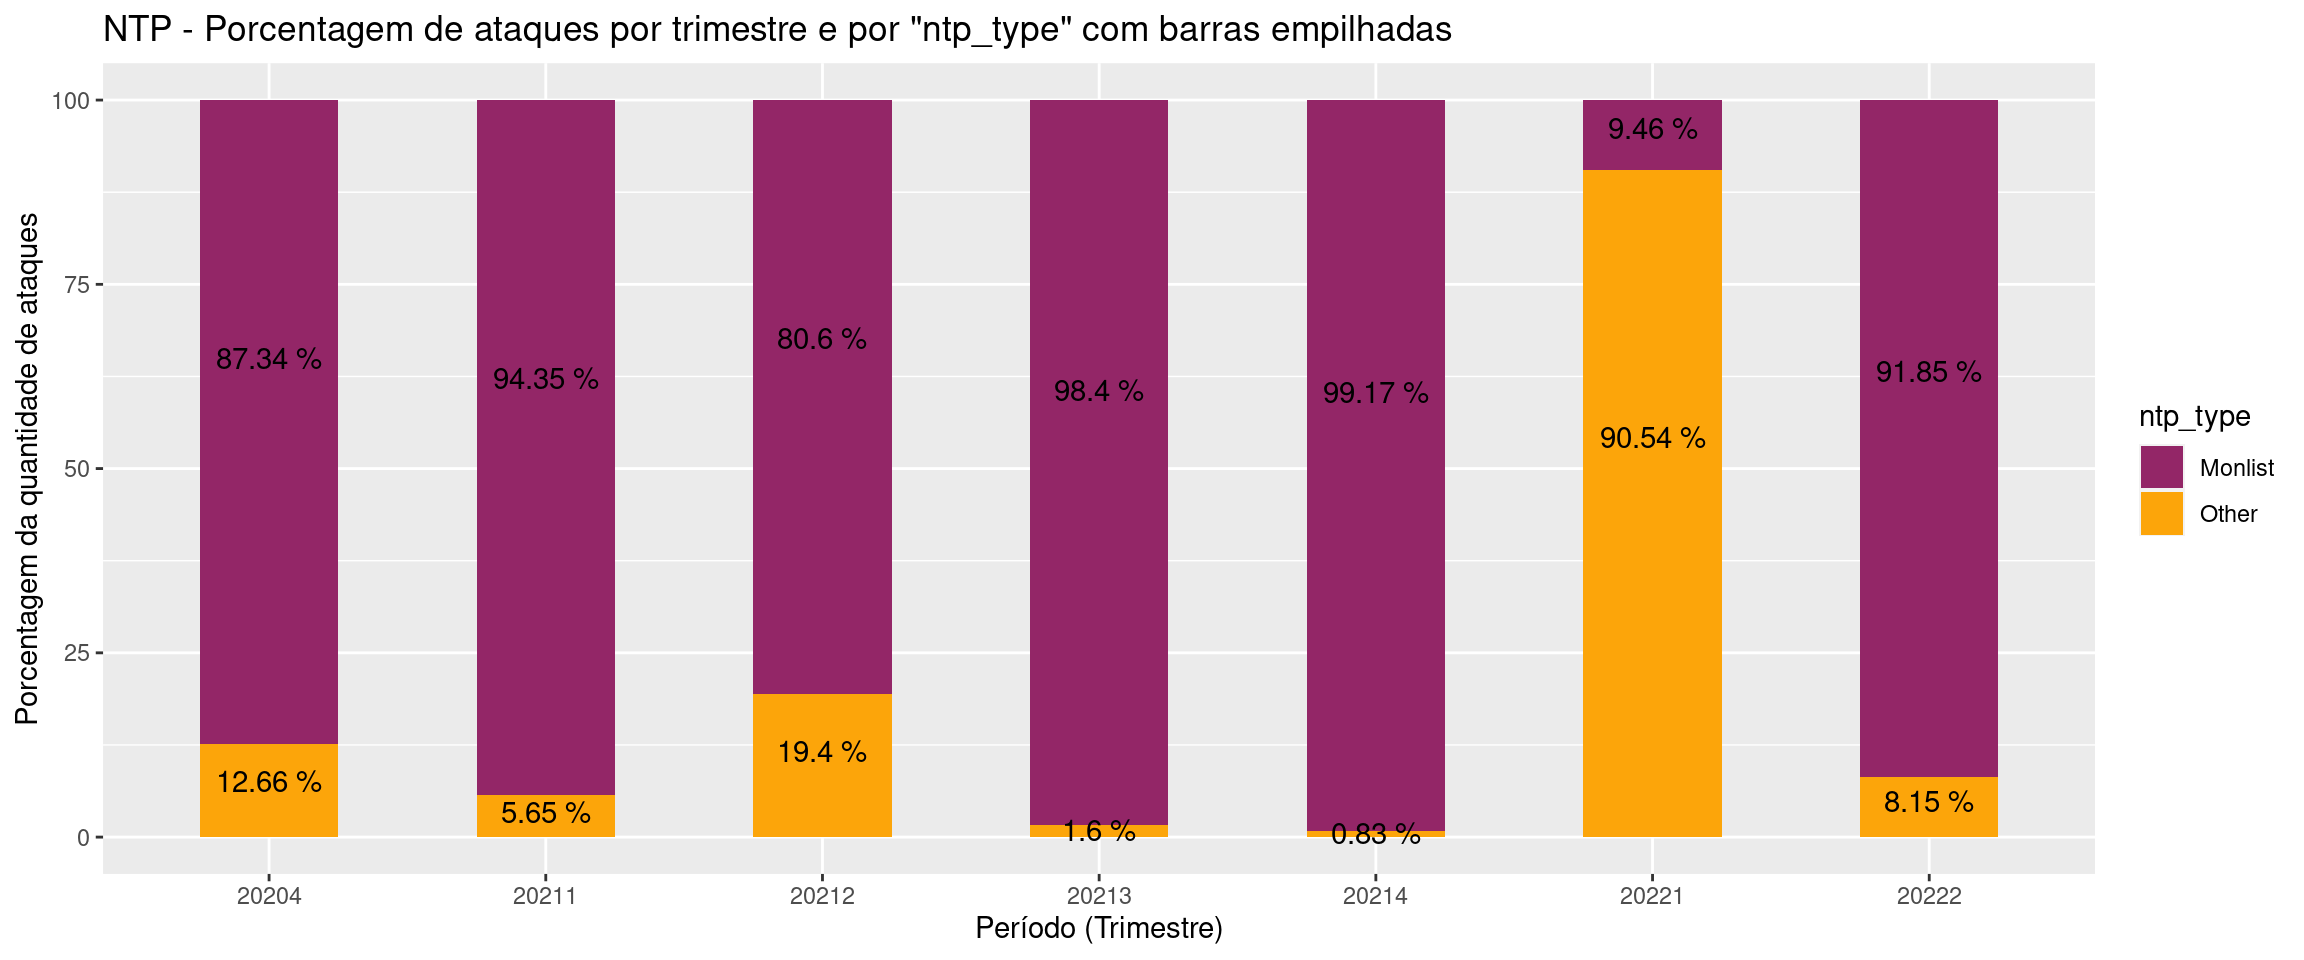
\includegraphics[width=0.75\linewidth]{ex-r-markdown_files/figure-latex/unnamed-chunk-3-1} \end{center}

\begin{itemize}
\tightlist
\item
  O peso do carro tende a prejudicar o consumo do carro, então qual mais
  pesado o carro, maior a probabilidade que o consumo do carro tenha um
  desempenho pior
\end{itemize}

\begin{enumerate}
\def\labelenumi{\arabic{enumi}.}
\setcounter{enumi}{6}
\tightlist
\item
  Resposta da questão 7
\end{enumerate}

\begin{Shaded}
\begin{Highlighting}[]
\FunctionTok{with}\NormalTok{(mtcars, }\FunctionTok{plot}\NormalTok{(mtcars}\SpecialCharTok{$}\NormalTok{gear, mtcars}\SpecialCharTok{$}\NormalTok{hp, }\AttributeTok{type =} \StringTok{\textquotesingle{}h\textquotesingle{}}\NormalTok{, }\AttributeTok{lwd =} \DecValTok{50}\NormalTok{))}
\end{Highlighting}
\end{Shaded}

\begin{center}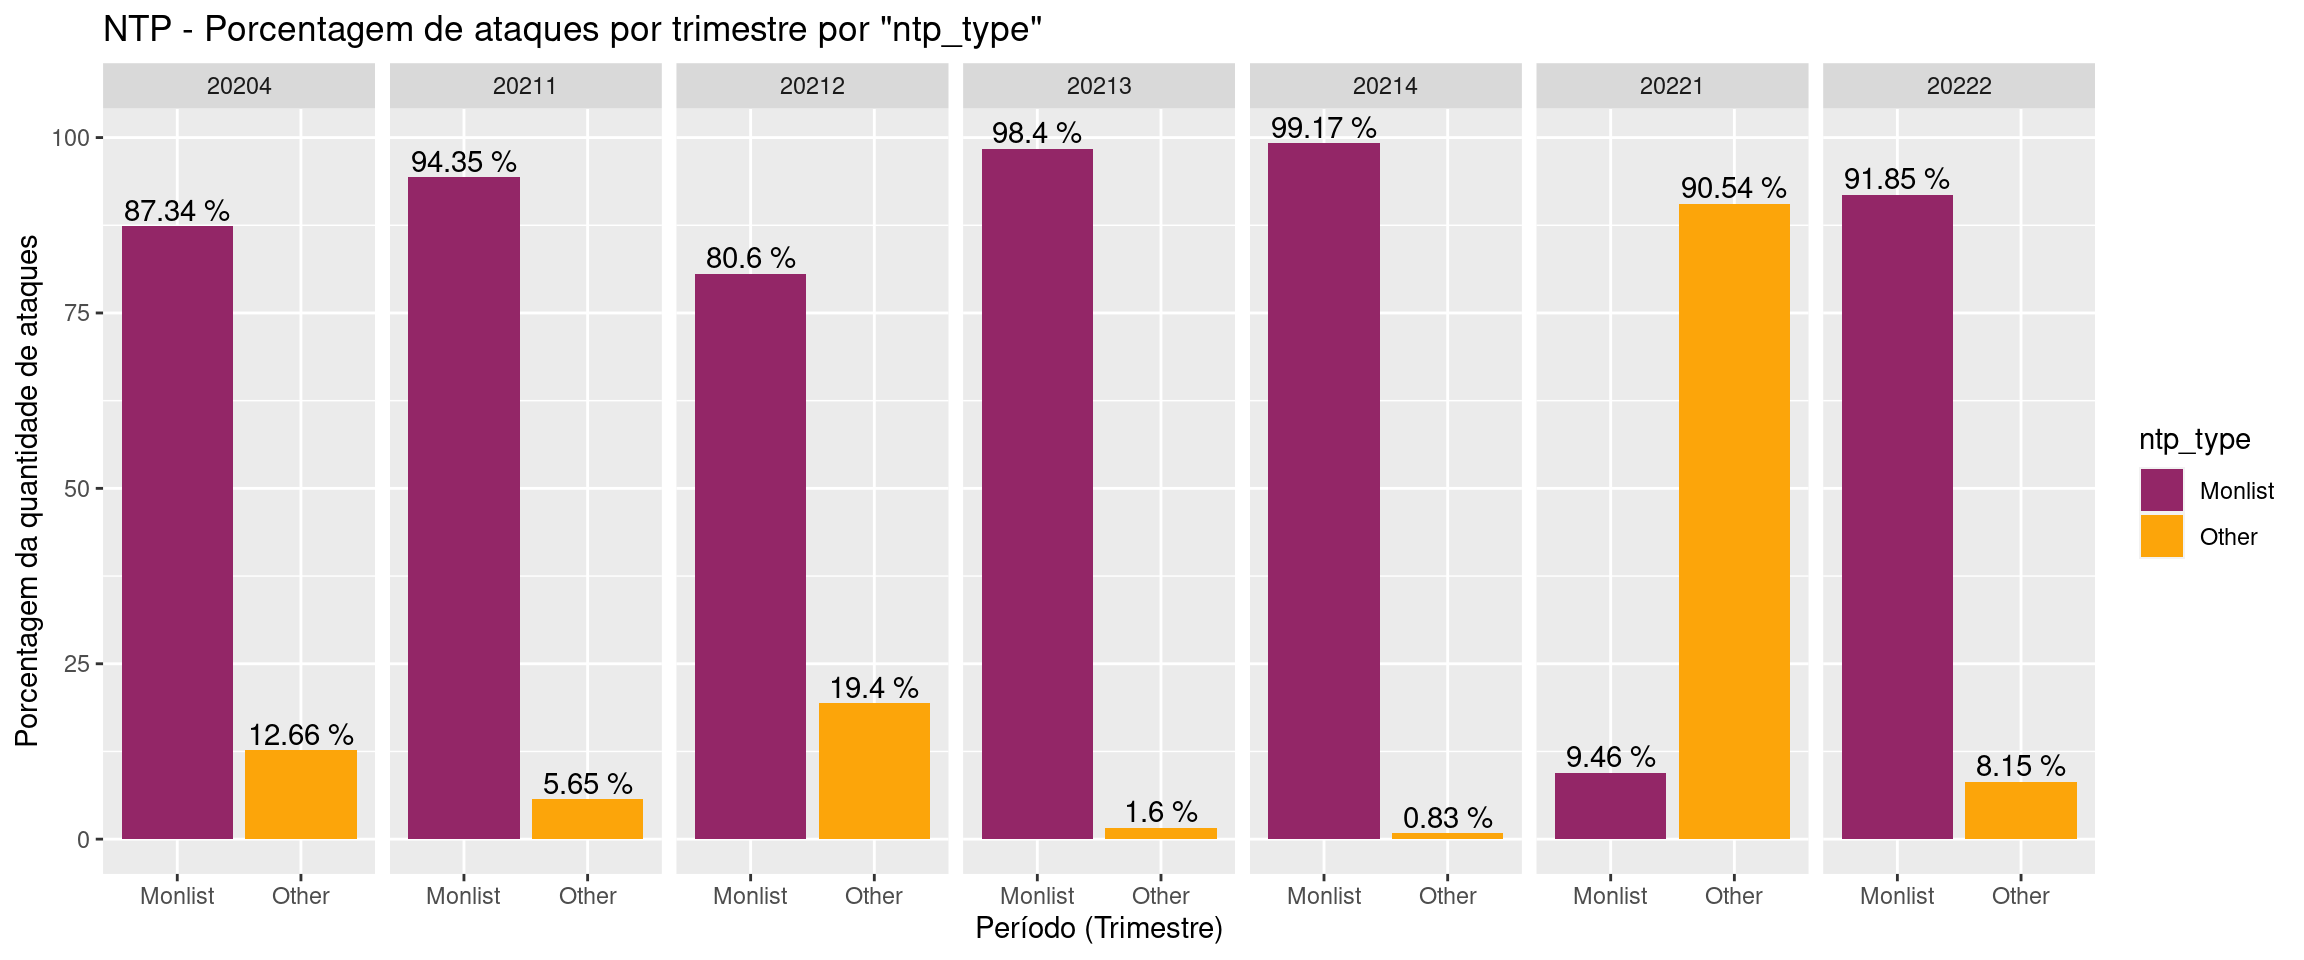
\includegraphics[width=0.75\linewidth]{ex-r-markdown_files/figure-latex/unnamed-chunk-4-1} \end{center}

\begin{itemize}
\tightlist
\item
  Na verdade, não é possível definir que carros com mais marchas tem
  mais potência no motor, pois temos carros com 3, 4, 5 marchas e na
  verdade, os carros com menor marchas 3 tem uma potência melhor que os
  4, mas os carros com uma potência de motor maior são os com 5
\end{itemize}

\hypertarget{anuxe1lise-do-conjunto-wwwusage}{%
\subsection{\texorpdfstring{Análise do conjunto
\texttt{WWWusage}}{Análise do conjunto WWWusage}}\label{anuxe1lise-do-conjunto-wwwusage}}

O conjunto \texttt{WWWusage} contém uma série de 100 medições do número
de usuários conectados à Internet através de um servidor a cada minuto.
Usando esse conjunto, responda às seguintes questões:

\begin{enumerate}
\def\labelenumi{\arabic{enumi}.}
\tightlist
\item
  Em que minuto o servidor teve a maior carga, e qual foi essa carga?
\item
  Em que minuto o servidor teve a menor carga, e qual foi essa carga?
\item
  Em que minuto o servidor teve o maior aumento de carga? Qual foi esse
  aumento (de quantos para quantos usuários)?
\item
  Em que minuto o servidor teve a maior redução de carga? Qual foi essa
  redução (de quantos para quantos usuários)?
\item
  Quantas vezes o número de usuários manteve-se constante em duas
  medições consecutivas?
\item
  Determine o número de usuários para o minuto 101, supondo que um
  eventual aumento ou redução de carga não ultrapasse os valores máximos
  obtidos nas questões 3 e 4. (Dica: você deverá estimar uma faixa de
  valores.)
\end{enumerate}

Código e saídas do R:

\begin{Shaded}
\begin{Highlighting}[]
\CommentTok{\# seu codigo R vai aqui}

\NormalTok{WWWusage.max }\OtherTok{\textless{}{-}} \FunctionTok{max}\NormalTok{(WWWusage)}
\NormalTok{WWWusage.max.which }\OtherTok{\textless{}{-}} \FunctionTok{which}\NormalTok{(WWWusage }\SpecialCharTok{==}\NormalTok{ WWWusage.max)}

\NormalTok{WWWusage.min }\OtherTok{\textless{}{-}} \FunctionTok{min}\NormalTok{(WWWusage)}
\NormalTok{WWWusage.min.which }\OtherTok{\textless{}{-}} \FunctionTok{which}\NormalTok{(WWWusage }\SpecialCharTok{==}\NormalTok{ WWWusage.min)}

\NormalTok{WWWusage.diff }\OtherTok{\textless{}{-}} \FunctionTok{diff}\NormalTok{(WWWusage)}
\NormalTok{WWWusage.diff.max }\OtherTok{\textless{}{-}} \FunctionTok{max}\NormalTok{(WWWusage.diff)}
\NormalTok{WWWusage.diff.max.which }\OtherTok{\textless{}{-}} \FunctionTok{which}\NormalTok{(WWWusage.diff }\SpecialCharTok{==}\NormalTok{ WWWusage.diff.max)}

\NormalTok{WWWusage.diff.min }\OtherTok{\textless{}{-}} \FunctionTok{min}\NormalTok{(WWWusage.diff)}
\NormalTok{WWWusage.diff.min.which }\OtherTok{\textless{}{-}} \FunctionTok{which}\NormalTok{(WWWusage.diff }\SpecialCharTok{==}\NormalTok{ WWWusage.diff.min)}

\NormalTok{WWWusage.diff.consecutive }\OtherTok{\textless{}{-}}\NormalTok{ WWWusage.diff[WWWusage.diff }\SpecialCharTok{==} \DecValTok{0}\NormalTok{]}
\NormalTok{WWWusage.last }\OtherTok{\textless{}{-}}\NormalTok{ WWWusage[}\FunctionTok{length}\NormalTok{(WWWusage)]}
  
\NormalTok{WWWusage.last.plusdif }\OtherTok{\textless{}{-}}\NormalTok{ WWWusage.last }\SpecialCharTok{+}\NormalTok{ WWWusage.diff.max}
\NormalTok{WWWusage.last.minusdif }\OtherTok{\textless{}{-}}\NormalTok{ WWWusage.last }\SpecialCharTok{{-}}\NormalTok{ WWWusage.diff.max}

\NormalTok{WWWusage.next.max }\OtherTok{\textless{}{-}} \FunctionTok{min}\NormalTok{(WWWusage.last.plusdif, WWWusage.max)}
\NormalTok{WWWusage.next.min }\OtherTok{\textless{}{-}} \FunctionTok{max}\NormalTok{(WWWusage.last.minusdif, WWWusage.min)}

\FunctionTok{summary}\NormalTok{(WWWusage)}
\end{Highlighting}
\end{Shaded}

\begin{verbatim}
##    Min. 1st Qu.  Median    Mean 3rd Qu.    Max. 
##    83.0    99.0   138.5   137.1   167.5   228.0
\end{verbatim}

\begin{Shaded}
\begin{Highlighting}[]
\FunctionTok{HoltWinters}\NormalTok{(WWWusage, }\AttributeTok{beta=}\ConstantTok{FALSE}\NormalTok{, }\AttributeTok{gamma=}\ConstantTok{FALSE}\NormalTok{)}
\end{Highlighting}
\end{Shaded}

\begin{verbatim}
## Holt-Winters exponential smoothing without trend and without seasonal component.
## 
## Call:
## HoltWinters(x = WWWusage, beta = FALSE, gamma = FALSE)
## 
## Smoothing parameters:
##  alpha: 0.99992
##  beta : FALSE
##  gamma: FALSE
## 
## Coefficients:
##       [,1]
## a 220.0002
\end{verbatim}

Respostas:

\begin{enumerate}
\def\labelenumi{\arabic{enumi}.}
\tightlist
\item
  Resposta da questão 1
\end{enumerate}

\begin{itemize}
\tightlist
\item
  No minuto 97 o servidor teve a maior carga de 228
\end{itemize}

\begin{enumerate}
\def\labelenumi{\arabic{enumi}.}
\setcounter{enumi}{1}
\tightlist
\item
  Resposta da questão 2
\end{enumerate}

\begin{itemize}
\tightlist
\item
  No minuto 7 o servidor teve a menor carga de 83
\end{itemize}

\begin{enumerate}
\def\labelenumi{\arabic{enumi}.}
\setcounter{enumi}{2}
\tightlist
\item
  Resposta da questão 3
\end{enumerate}

\begin{itemize}
\tightlist
\item
  Nos minutos 14, 81 para os 15, 82 teve um aumento de 14 usuários
\end{itemize}

\begin{enumerate}
\def\labelenumi{\arabic{enumi}.}
\setcounter{enumi}{3}
\tightlist
\item
  Resposta da questão 4
\end{enumerate}

\begin{itemize}
\tightlist
\item
  No minuto 57 para o minuto 58 teve uma redução de 14 usuários
\end{itemize}

\begin{enumerate}
\def\labelenumi{\arabic{enumi}.}
\setcounter{enumi}{4}
\tightlist
\item
  Resposta da questão 5
\end{enumerate}

\begin{itemize}
\tightlist
\item
  9 vezes o número de usuários manteve-se com duas medições consecutivas
\end{itemize}

\begin{enumerate}
\def\labelenumi{\arabic{enumi}.}
\setcounter{enumi}{5}
\tightlist
\item
  Resposta da questão 6
\end{enumerate}

\begin{Shaded}
\begin{Highlighting}[]
\FunctionTok{plot}\NormalTok{(WWWusage)}
\end{Highlighting}
\end{Shaded}

\begin{center}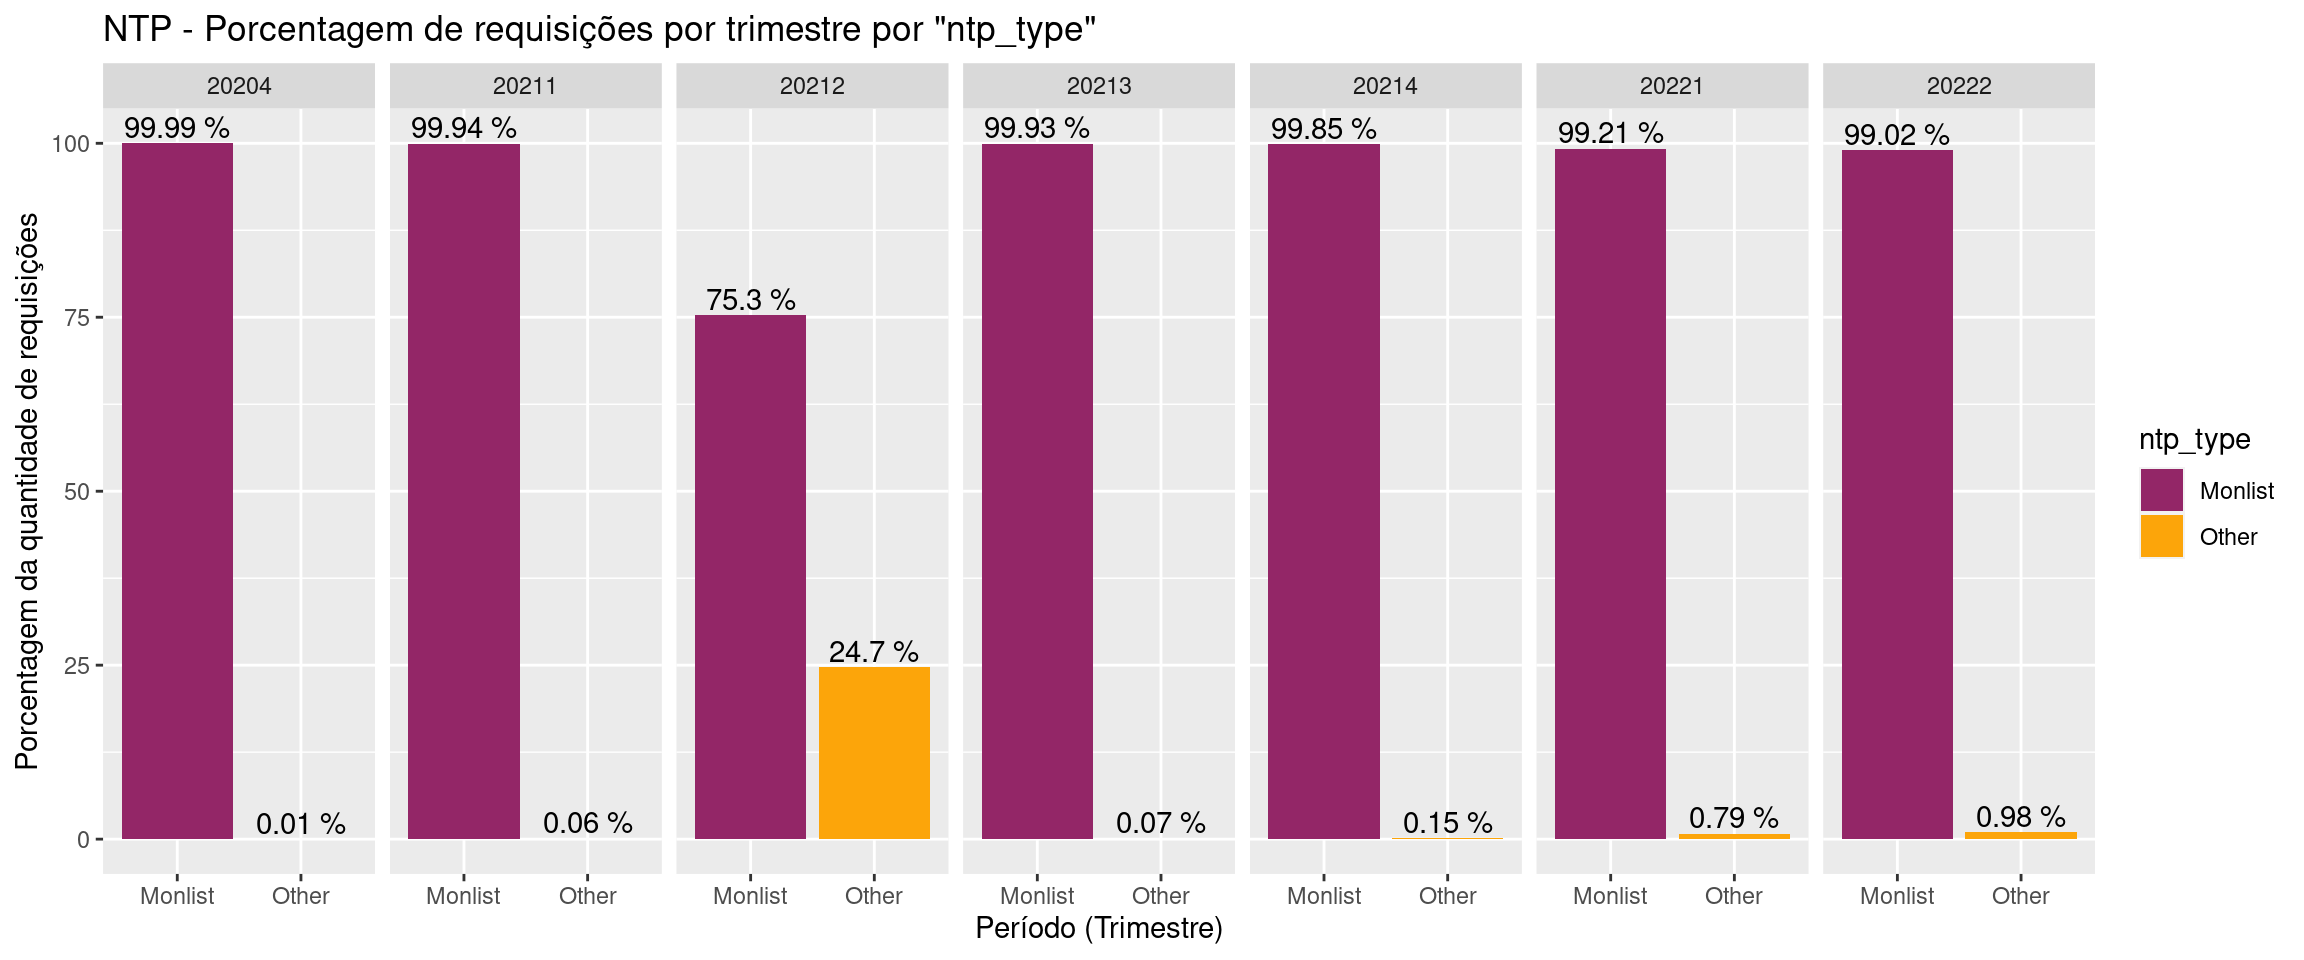
\includegraphics[width=0.75\linewidth]{ex-r-markdown_files/figure-latex/unnamed-chunk-5-1} \end{center}

\begin{itemize}
\tightlist
\item
  Para estimar o numero de usuarios para o minuto 101, levando em
  consideração o maior aumento de usuários ja registrado 14 entre um
  minuto e outro e o ultimo valor registrado de 220 usuários, e também a
  mínima 83 e máxima 228, o range provável do minuto 101 será entre 206
  e 228.
\item
  Ja HoltWinters estima o seguinte valor:
\end{itemize}

\begin{Shaded}
\begin{Highlighting}[]
\FunctionTok{HoltWinters}\NormalTok{(WWWusage, }\AttributeTok{beta=}\ConstantTok{FALSE}\NormalTok{, }\AttributeTok{gamma=}\ConstantTok{FALSE}\NormalTok{)}
\end{Highlighting}
\end{Shaded}

\begin{verbatim}
## Holt-Winters exponential smoothing without trend and without seasonal component.
## 
## Call:
## HoltWinters(x = WWWusage, beta = FALSE, gamma = FALSE)
## 
## Smoothing parameters:
##  alpha: 0.99992
##  beta : FALSE
##  gamma: FALSE
## 
## Coefficients:
##       [,1]
## a 220.0002
\end{verbatim}

\end{document}
